% Options for packages loaded elsewhere
\PassOptionsToPackage{unicode}{hyperref}
\PassOptionsToPackage{hyphens}{url}
\PassOptionsToPackage{dvipsnames,svgnames,x11names}{xcolor}
%
\documentclass[
  letterpaper,
  DIV=11,
  numbers=noendperiod]{scrartcl}

\usepackage{amsmath,amssymb}
\usepackage{lmodern}
\usepackage{iftex}
\ifPDFTeX
  \usepackage[T1]{fontenc}
  \usepackage[utf8]{inputenc}
  \usepackage{textcomp} % provide euro and other symbols
\else % if luatex or xetex
  \usepackage{unicode-math}
  \defaultfontfeatures{Scale=MatchLowercase}
  \defaultfontfeatures[\rmfamily]{Ligatures=TeX,Scale=1}
\fi
% Use upquote if available, for straight quotes in verbatim environments
\IfFileExists{upquote.sty}{\usepackage{upquote}}{}
\IfFileExists{microtype.sty}{% use microtype if available
  \usepackage[]{microtype}
  \UseMicrotypeSet[protrusion]{basicmath} % disable protrusion for tt fonts
}{}
\makeatletter
\@ifundefined{KOMAClassName}{% if non-KOMA class
  \IfFileExists{parskip.sty}{%
    \usepackage{parskip}
  }{% else
    \setlength{\parindent}{0pt}
    \setlength{\parskip}{6pt plus 2pt minus 1pt}}
}{% if KOMA class
  \KOMAoptions{parskip=half}}
\makeatother
\usepackage{xcolor}
\setlength{\emergencystretch}{3em} % prevent overfull lines
\setcounter{secnumdepth}{5}
% Make \paragraph and \subparagraph free-standing
\ifx\paragraph\undefined\else
  \let\oldparagraph\paragraph
  \renewcommand{\paragraph}[1]{\oldparagraph{#1}\mbox{}}
\fi
\ifx\subparagraph\undefined\else
  \let\oldsubparagraph\subparagraph
  \renewcommand{\subparagraph}[1]{\oldsubparagraph{#1}\mbox{}}
\fi

\usepackage{color}
\usepackage{fancyvrb}
\newcommand{\VerbBar}{|}
\newcommand{\VERB}{\Verb[commandchars=\\\{\}]}
\DefineVerbatimEnvironment{Highlighting}{Verbatim}{commandchars=\\\{\}}
% Add ',fontsize=\small' for more characters per line
\usepackage{framed}
\definecolor{shadecolor}{RGB}{241,243,245}
\newenvironment{Shaded}{\begin{snugshade}}{\end{snugshade}}
\newcommand{\AlertTok}[1]{\textcolor[rgb]{0.68,0.00,0.00}{#1}}
\newcommand{\AnnotationTok}[1]{\textcolor[rgb]{0.37,0.37,0.37}{#1}}
\newcommand{\AttributeTok}[1]{\textcolor[rgb]{0.40,0.45,0.13}{#1}}
\newcommand{\BaseNTok}[1]{\textcolor[rgb]{0.68,0.00,0.00}{#1}}
\newcommand{\BuiltInTok}[1]{\textcolor[rgb]{0.00,0.23,0.31}{#1}}
\newcommand{\CharTok}[1]{\textcolor[rgb]{0.13,0.47,0.30}{#1}}
\newcommand{\CommentTok}[1]{\textcolor[rgb]{0.37,0.37,0.37}{#1}}
\newcommand{\CommentVarTok}[1]{\textcolor[rgb]{0.37,0.37,0.37}{\textit{#1}}}
\newcommand{\ConstantTok}[1]{\textcolor[rgb]{0.56,0.35,0.01}{#1}}
\newcommand{\ControlFlowTok}[1]{\textcolor[rgb]{0.00,0.23,0.31}{#1}}
\newcommand{\DataTypeTok}[1]{\textcolor[rgb]{0.68,0.00,0.00}{#1}}
\newcommand{\DecValTok}[1]{\textcolor[rgb]{0.68,0.00,0.00}{#1}}
\newcommand{\DocumentationTok}[1]{\textcolor[rgb]{0.37,0.37,0.37}{\textit{#1}}}
\newcommand{\ErrorTok}[1]{\textcolor[rgb]{0.68,0.00,0.00}{#1}}
\newcommand{\ExtensionTok}[1]{\textcolor[rgb]{0.00,0.23,0.31}{#1}}
\newcommand{\FloatTok}[1]{\textcolor[rgb]{0.68,0.00,0.00}{#1}}
\newcommand{\FunctionTok}[1]{\textcolor[rgb]{0.28,0.35,0.67}{#1}}
\newcommand{\ImportTok}[1]{\textcolor[rgb]{0.00,0.46,0.62}{#1}}
\newcommand{\InformationTok}[1]{\textcolor[rgb]{0.37,0.37,0.37}{#1}}
\newcommand{\KeywordTok}[1]{\textcolor[rgb]{0.00,0.23,0.31}{#1}}
\newcommand{\NormalTok}[1]{\textcolor[rgb]{0.00,0.23,0.31}{#1}}
\newcommand{\OperatorTok}[1]{\textcolor[rgb]{0.37,0.37,0.37}{#1}}
\newcommand{\OtherTok}[1]{\textcolor[rgb]{0.00,0.23,0.31}{#1}}
\newcommand{\PreprocessorTok}[1]{\textcolor[rgb]{0.68,0.00,0.00}{#1}}
\newcommand{\RegionMarkerTok}[1]{\textcolor[rgb]{0.00,0.23,0.31}{#1}}
\newcommand{\SpecialCharTok}[1]{\textcolor[rgb]{0.37,0.37,0.37}{#1}}
\newcommand{\SpecialStringTok}[1]{\textcolor[rgb]{0.13,0.47,0.30}{#1}}
\newcommand{\StringTok}[1]{\textcolor[rgb]{0.13,0.47,0.30}{#1}}
\newcommand{\VariableTok}[1]{\textcolor[rgb]{0.07,0.07,0.07}{#1}}
\newcommand{\VerbatimStringTok}[1]{\textcolor[rgb]{0.13,0.47,0.30}{#1}}
\newcommand{\WarningTok}[1]{\textcolor[rgb]{0.37,0.37,0.37}{\textit{#1}}}

\providecommand{\tightlist}{%
  \setlength{\itemsep}{0pt}\setlength{\parskip}{0pt}}\usepackage{longtable,booktabs,array}
\usepackage{calc} % for calculating minipage widths
% Correct order of tables after \paragraph or \subparagraph
\usepackage{etoolbox}
\makeatletter
\patchcmd\longtable{\par}{\if@noskipsec\mbox{}\fi\par}{}{}
\makeatother
% Allow footnotes in longtable head/foot
\IfFileExists{footnotehyper.sty}{\usepackage{footnotehyper}}{\usepackage{footnote}}
\makesavenoteenv{longtable}
\usepackage{graphicx}
\makeatletter
\def\maxwidth{\ifdim\Gin@nat@width>\linewidth\linewidth\else\Gin@nat@width\fi}
\def\maxheight{\ifdim\Gin@nat@height>\textheight\textheight\else\Gin@nat@height\fi}
\makeatother
% Scale images if necessary, so that they will not overflow the page
% margins by default, and it is still possible to overwrite the defaults
% using explicit options in \includegraphics[width, height, ...]{}
\setkeys{Gin}{width=\maxwidth,height=\maxheight,keepaspectratio}
% Set default figure placement to htbp
\makeatletter
\def\fps@figure{htbp}
\makeatother

\KOMAoption{captions}{tableheading}
\makeatletter
\makeatother
\makeatletter
\makeatother
\makeatletter
\@ifpackageloaded{caption}{}{\usepackage{caption}}
\AtBeginDocument{%
\ifdefined\contentsname
  \renewcommand*\contentsname{Table of contents}
\else
  \newcommand\contentsname{Table of contents}
\fi
\ifdefined\listfigurename
  \renewcommand*\listfigurename{List of Figures}
\else
  \newcommand\listfigurename{List of Figures}
\fi
\ifdefined\listtablename
  \renewcommand*\listtablename{List of Tables}
\else
  \newcommand\listtablename{List of Tables}
\fi
\ifdefined\figurename
  \renewcommand*\figurename{Figure}
\else
  \newcommand\figurename{Figure}
\fi
\ifdefined\tablename
  \renewcommand*\tablename{Table}
\else
  \newcommand\tablename{Table}
\fi
}
\@ifpackageloaded{float}{}{\usepackage{float}}
\floatstyle{ruled}
\@ifundefined{c@chapter}{\newfloat{codelisting}{h}{lop}}{\newfloat{codelisting}{h}{lop}[chapter]}
\floatname{codelisting}{Listing}
\newcommand*\listoflistings{\listof{codelisting}{List of Listings}}
\makeatother
\makeatletter
\@ifpackageloaded{caption}{}{\usepackage{caption}}
\@ifpackageloaded{subcaption}{}{\usepackage{subcaption}}
\makeatother
\makeatletter
\@ifpackageloaded{tcolorbox}{}{\usepackage[many]{tcolorbox}}
\makeatother
\makeatletter
\@ifundefined{shadecolor}{\definecolor{shadecolor}{rgb}{.97, .97, .97}}
\makeatother
\makeatletter
\makeatother
\ifLuaTeX
  \usepackage{selnolig}  % disable illegal ligatures
\fi
\IfFileExists{bookmark.sty}{\usepackage{bookmark}}{\usepackage{hyperref}}
\IfFileExists{xurl.sty}{\usepackage{xurl}}{} % add URL line breaks if available
\urlstyle{same} % disable monospaced font for URLs
\hypersetup{
  pdftitle={Project Report},
  pdfauthor={Hiba Khatib, Emily Leibfritz, Nicole Birova, and YuYan Zhang},
  colorlinks=true,
  linkcolor={blue},
  filecolor={Maroon},
  citecolor={Blue},
  urlcolor={Blue},
  pdfcreator={LaTeX via pandoc}}

\title{Project Report}
\usepackage{etoolbox}
\makeatletter
\providecommand{\subtitle}[1]{% add subtitle to \maketitle
  \apptocmd{\@title}{\par {\large #1 \par}}{}{}
}
\makeatother
\subtitle{dat\_sci}
\author{Hiba Khatib, Emily Leibfritz, Nicole Birova, and YuYan Zhang}
\date{05/23/2023}

\begin{document}
\maketitle
\begin{abstract}
\emph{The ABSTRACT is to be in fully-justified italicized text at the
top of the report, below the author information. The abstract section
must summarise the problem statement, the developed model(s), the
metric(s) optimized and the recommendations to the stakeholders based on
the model (if any). You may also briefly mention any major EDA-based
insights that helped develop the model or directly translated into
recommendations to the stakeholders. However, the abstract must not be
more than 200 words in length}.
\end{abstract}
\ifdefined\Shaded\renewenvironment{Shaded}{\begin{tcolorbox}[frame hidden, boxrule=0pt, interior hidden, breakable, borderline west={3pt}{0pt}{shadecolor}, sharp corners, enhanced]}{\end{tcolorbox}}\fi

\hypertarget{background-motivation}{%
\subsection{Background / Motivation}\label{background-motivation}}

Since buying a used car requires a level of trust between buyers and
sellers, it's difficult to know what a good price is. We want to make a
tool that buyers and sellers can use to facilitate the exchange.

This is also useful for us as college students and young people in the
workforce with limited budgets but a need for a vehicle.

\hypertarget{problem-statement}{%
\subsection{Problem statement}\label{problem-statement}}

The car industry is vast, and venturing into buying or selling a car can
often be challenging, especially as the used car market is even harder
to keep track off. Therefore, we want to create a model that can give
potential buyers and sellers on overview of what to expect in price
range.

\hypertarget{data-sources}{%
\subsection{Data sources}\label{data-sources}}

\emph{by Hiba Khatib}

The data we used is from Kaggle
https://www.kaggle.com/datasets/ananaymital/us-used-cars-dataset. The
original dataset has 3 million observations but we randomly sampled 6000
observations to used as our test and train data. This will help solve
the problem because as it containts the price as well as
\textasciitilde50 other charactersitics describing cars that were sold
used. From this data, we can build a model predicting car price to help
potential sellers adjust heir expectations and potential buyers to get a
reasonable price range for the car they are expecting to buy.

\hypertarget{stakeholders}{%
\subsection{Stakeholders}\label{stakeholders}}

Who cares? If you are successful, what difference will it make to them?

\emph{by Hiba Khatib}

Our stakeholders are used car buyers, seller, and third-parties that
enable these exchanges.

Understanding the used cars market is important for several reasons, and
developing a machine learning tool that predicts the price of a used car
can be valuable for both individuals and used car dealerships. Here are
some ways that our tool is significant:

\begin{enumerate}
\def\labelenumi{\arabic{enumi}.}
\item
  \textbf{Informed Decision-Making:} For individuals looking to buy or
  sell a used car, having knowledge about the current market conditions,
  trends, and prices is crucial. Understanding the used cars market
  allows buyers to make informed decisions regarding the fair value of a
  vehicle they are interested in purchasing. Similarly, sellers can
  accurately assess the appropriate price to ask for their used car,
  ensuring they receive a fair deal.
\item
  \textbf{Fair Pricing:} Predicting the price of a used car using
  machine learning can help establish fair and reasonable prices for
  both buyers and sellers. By considering various factors such as the
  car's make, model, year, mileage, and condition, our can provide an
  estimate that aligns with the prevailing market rates. This promotes
  transparency and prevents unfair price manipulation.
\item
  \textbf{Time and Cost Savings:} For buyers, a machine learning tool
  can save time and effort by quickly providing estimated prices for a
  wide range of used cars. Instead of manually researching and comparing
  prices, potential buyers can use the tool to narrow down their options
  and focus on vehicles within their budget. For sellers, having a
  reliable price prediction tool eliminates the need for extensive
  market research and allows them to set competitive prices efficiently.
\item
  \textbf{Negotiation Power:} When buying or selling a used car,
  negotiations are often involved. Having access to a machine learning
  tool that predicts prices empowers both parties during the negotiation
  process. Buyers can negotiate based on market insights, ensuring they
  are not overpaying, while sellers can justify their asking price with
  data-driven estimates.
\item
  \textbf{Business Optimization:} Used car dealerships can greatly
  benefit from a machine learning tool that predicts prices. It allows
  dealerships to assess the value of trade-ins accurately, determine
  competitive pricing strategies, and optimize inventory management. By
  understanding market trends and fluctuations, dealerships can make
  informed decisions that maximize profitability and customer
  satisfaction.
\item
  \textbf{Risk Mitigation:} Predicting the price of used cars can also
  help mitigate risk for both buyers and sellers. Buyers can avoid
  purchasing a vehicle at an inflated price by comparing the predicted
  price with the seller's offer. Sellers, on the other hand, can ensure
  they do not undervalue their vehicles and receive fair compensation
  for their assets.
\end{enumerate}

Overall, understanding the used cars market and having a machine
learning tool to predict prices is beneficial for individuals and used
car dealerships. It facilitates informed decision-making, establishes
fair pricing, saves time and effort, enhances negotiation power,
optimizes business operations, and mitigates risks in the used car
market.

\hypertarget{data-quality-check-cleaning-preparation}{%
\subsection{Data quality check / cleaning /
preparation}\label{data-quality-check-cleaning-preparation}}

\emph{Written by Hiba Khatib; code and data cleaning process done by
both Hiba Khatib \& Emily Leibfritz}

\begin{verbatim}
The standard deviation of the target variable before removing outliers 16742.99685916766
The mean of the target variable before removing outliers 24568.3835
\end{verbatim}

\begin{verbatim}
C:\Users\hibar\anaconda3\lib\site-packages\seaborn\_decorators.py:36: FutureWarning: Pass the following variable as a keyword arg: x. From version 0.12, the only valid positional argument will be `data`, and passing other arguments without an explicit keyword will result in an error or misinterpretation.
  warnings.warn(
\end{verbatim}

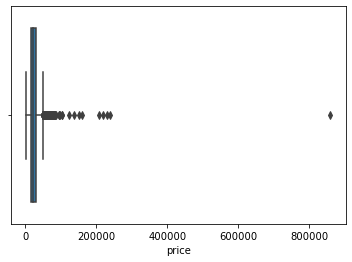
\includegraphics{Final Project Report - Used Cars Regression_files/figure-pdf/cell-3-output-3.png}

\begin{verbatim}
C:\Users\hibar\anaconda3\lib\site-packages\seaborn\_decorators.py:36: FutureWarning: Pass the following variable as a keyword arg: x. From version 0.12, the only valid positional argument will be `data`, and passing other arguments without an explicit keyword will result in an error or misinterpretation.
  warnings.warn(
\end{verbatim}

\begin{verbatim}
<AxesSubplot:xlabel='price'>
\end{verbatim}

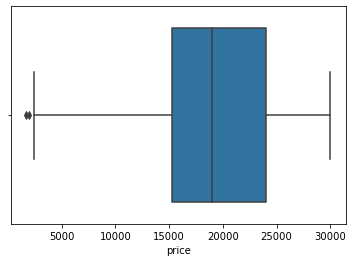
\includegraphics{Final Project Report - Used Cars Regression_files/figure-pdf/cell-4-output-3.png}

\begin{verbatim}
Mean of target price after dropping outliers:  19205.211827007945
Standard deviation:  5978.306973568847
\end{verbatim}

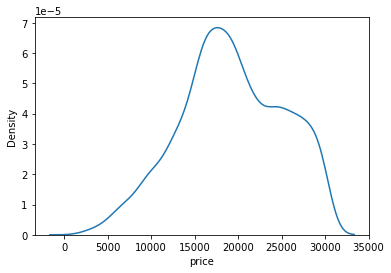
\includegraphics{Final Project Report - Used Cars Regression_files/figure-pdf/cell-5-output-2.png}

\begin{Shaded}
\begin{Highlighting}[]
\CommentTok{\#\#\# Distribution of most significant predictors}
\CommentTok{\# the following code was done by Emily Leibfritz}
\ImportTok{import}\NormalTok{ seaborn }\ImportTok{as}\NormalTok{ sns}
\end{Highlighting}
\end{Shaded}

\begin{verbatim}
[]
\end{verbatim}

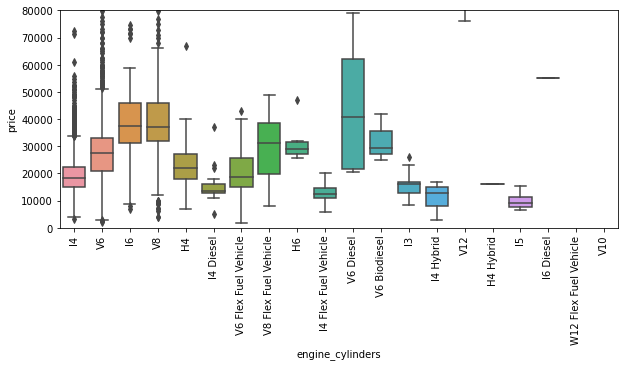
\includegraphics{Final Project Report - Used Cars Regression_files/figure-pdf/cell-7-output-2.png}

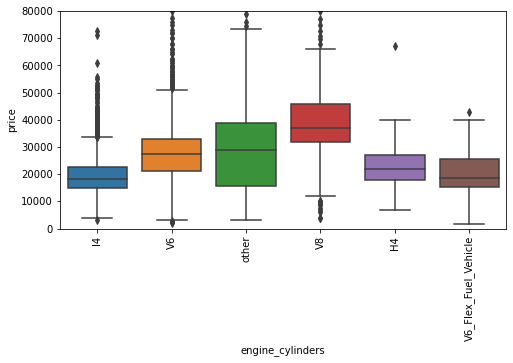
\includegraphics{Final Project Report - Used Cars Regression_files/figure-pdf/cell-7-output-3.png}

\begin{verbatim}
[]
\end{verbatim}

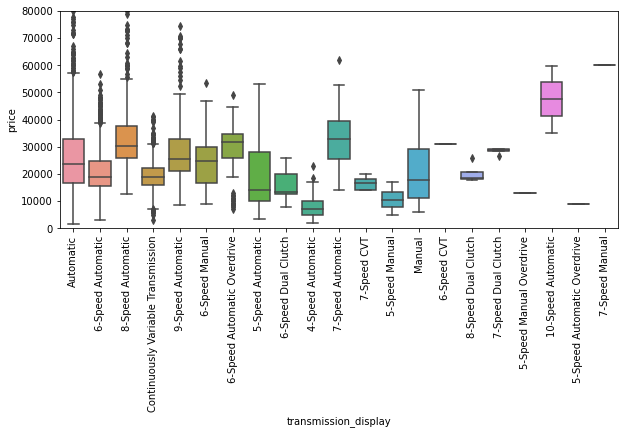
\includegraphics{Final Project Report - Used Cars Regression_files/figure-pdf/cell-8-output-2.png}

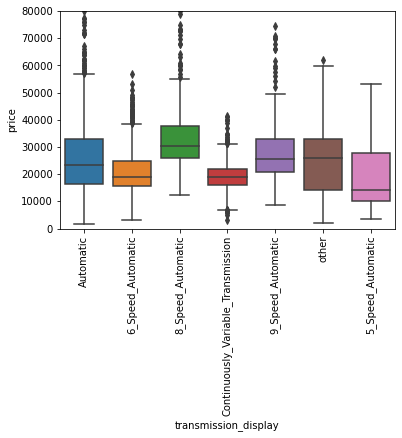
\includegraphics{Final Project Report - Used Cars Regression_files/figure-pdf/cell-8-output-3.png}

\begin{longtable}[]{@{}llllllllllllllllllllll@{}}
\toprule()
& city\_fuel\_economy & engine\_displacement & franchise\_make &
fuel\_tank\_volume & height & highway\_fuel\_economy & length & mileage
& model\_name & owner\_count & ... & trimId & wheelbase & width & year &
wheel\_system\_cat & wheel\_system\_display\_cat & body\_type\_Sedan &
engine\_cylinders\_I4 & engine\_cylinders\_V6 &
transmission\_display\_8\_Speed\_Automatic \\
\midrule()
\endhead
count & 4531.000000 & 4531.000000 & 4531.000000 & 4531.000000 &
4531.00000 & 4531.000000 & 4531.000000 & 4531.000000 & 4531.000000 &
4531.000000 & ... & 4531.000000 & 4531.000000 & 4531.000000 &
4531.000000 & 4531.000000 & 4531.000000 & 4531.000000 & 4531.000000 &
4531.000000 & 4531.000000 \\
mean & 22.123814 & 2653.520194 & 0.976826 & 17.239881 & 63.71748 &
29.835356 & 187.880755 & 50587.295299 & 1.203708 & 1.374752 & ... &
66545.237696 & 110.453719 & 76.634937 & 2016.423085 & 2.440742 &
2.348267 & 0.331494 & 0.612668 & 0.269918 & 0.073714 \\
std & 4.370368 & 889.783980 & 1.181402 & 3.710306 & 5.77055 & 5.156303 &
12.964924 & 38325.667183 & 0.804647 & 0.699996 & ... & 14455.076888 &
8.196206 & 6.360904 & 2.846164 & 0.998325 & 1.004233 & 0.470802 &
0.487194 & 0.443966 & 0.261334 \\
min & 11.000000 & 1000.000000 & 0.000000 & 9.200000 & 47.30000 &
15.000000 & 144.700000 & 10.000000 & 0.000000 & 1.000000 & ... &
297.000000 & 90.900000 & 62.900000 & 1993.000000 & 0.000000 & 0.000000 &
0.000000 & 0.000000 & 0.000000 & 0.000000 \\
25\% & 19.000000 & 2000.000000 & 0.000000 & 14.500000 & 57.90000 &
26.000000 & 180.550000 & 25122.500000 & 1.000000 & 1.000000 & ... &
57983.000000 & 105.900000 & 72.300000 & 2016.000000 & 2.000000 &
1.000000 & 0.000000 & 0.000000 & 0.000000 & 0.000000 \\
50\% & 22.000000 & 2400.000000 & 1.000000 & 16.500000 & 65.40000 &
30.000000 & 187.400000 & 38403.000000 & 1.000000 & 1.000000 & ... &
68658.000000 & 109.300000 & 73.400000 & 2017.000000 & 3.000000 &
3.000000 & 0.000000 & 1.000000 & 0.000000 & 0.000000 \\
75\% & 25.000000 & 3500.000000 & 1.000000 & 19.000000 & 67.90000 &
34.000000 & 192.900000 & 66451.000000 & 2.000000 & 2.000000 & ... &
76471.500000 & 112.500000 & 81.300000 & 2018.000000 & 3.000000 &
3.000000 & 1.000000 & 1.000000 & 1.000000 & 0.000000 \\
max & 37.000000 & 6200.000000 & 4.000000 & 36.000000 & 108.60000 &
43.000000 & 250.400000 & 294140.000000 & 4.000000 & 8.000000 & ... &
92998.000000 & 164.600000 & 97.400000 & 2020.000000 & 4.000000 &
4.000000 & 1.000000 & 1.000000 & 1.000000 & 1.000000 \\
\bottomrule()
\end{longtable}

This is a summary of our main takeaways from the data prep and EDA:

\begin{itemize}
\item
  The first thing we did was fix the data types of some of the columns.
  All of the boolean columns were encoded as True or False so we mapped
  those to 1s and 0s. Then, we found that several columns such as
  horsepower and torque were numerical but contained units. We removed
  all of the units from these columns and converted them back to
  numeric.
\item
  Then, we dropped a set of unique identifiers which were not sigificant
  to our analysis. We also dropped three columns which represented the
  interior, and exterior color of the car. These columns had different
  names for the same color and we did not see them as significant
  predictors to engineer and encode differently.
\item
  Then, we dropped a constant predictor which contained the same value
  for all observations as constant predictors don't provide any
  meaningful insights.
\item
  The final step in the cleaning and preparation of the numerical data,
  we dropped highly correlated features. These were features which
  represented the same information in two different ways such as the
  official name of a trim and the id associated with that name. This
  resulted in us keeping only 14 of the numerical predictors are
  subsetting for predictors with a correlation of \textbar-.2\textbar.
\item
  For the categorical columns, each was observed individually in order
  to find the best way to handle them, as just converting them all into
  dummies resulted in a huge dataset.
\item
  Some columns with few unique values that showed a connection to the
  target variable were just converted into dummies, like body\_type and
  transmission\_display.
\item
  Some columns, like engine\_cylinders and transmission display had some
  values very common while others only had under 100 observations. These
  were grouped as others, and the columns were converted into dummies.
\item
  Some columns like franchise\_make and model\_name had a too large
  amount of unique values to convert into dummies, so the observations
  were grouped by mean value of target variable, and assigned a number
  between 1-6.
\item
  Some columns did not show any connection to the target variable, while
  often having a big amount of unique values, like the columns
  concerning the color of the vehicles, city or major\_options. These
  columns were dropped.
\item
  Some columns contained the same information given by other columns
  already, like the pairs trim\&trimID, make\_name\&franchise\_make,
  engine\_type\&engine\_cylinders where each trim, engine\_type and
  make\_name were dropped.
\end{itemize}

\hypertarget{exploratory-data-analysis}{%
\subsection{Exploratory data analysis}\label{exploratory-data-analysis}}

\emph{Written by Hiba Khatib; EDA code was written by Hiba Khatib \&
Emily Leibfritz}

The main takeaway from the EDA was the way that some columns were
encoded. Some of the numerical columns had units. We had to remove the
units in order to truly observe the trends in the numerical data.
Additionally, the most important takeaway was the outliers and their
effects on the distribution of the data. We intially focused only on the
plot of the target variable which indicated that a log transformation
was necessary but after dropping the outliers, the target no longer
required a transformation.

We did not have missing data except for one observation. When I sampled
the data from the original 3 million observation data set, I achieved a
subset of the data with no missing values. One observation later caused
issues because some of its columns had dashes -- instead of NaN or empty
cells. After we performed data cleaning, this observation's missingness
becamse apparent. We dropped this observation since it was one out of
4500+ observations and was not worth imputing.

Please refer to the graphs above to explore some of our EDA and data
prep. The project code contains extensive data cleaning and EDA which
can not reasonably be included in the report.

\hypertarget{feature-selection}{%
\subsection{Feature Selection}\label{feature-selection}}

\emph{By Hiba Khatib}

I performed two main sets of feature selection as I later discuss in my
MARS and Random Forest models. Below, I outlined some reasons as to why
several methods of feature selection can be very beneficial for machine
learning models:

\begin{enumerate}
\def\labelenumi{\arabic{enumi}.}
\item
  Robustness and Reliability: Using multiple feature selection
  techniques helps ensure the robustness and reliability of our ultimate
  machine learning model. Different feature selection methods have their
  own strengths and weaknesses, and by employing two distinct
  approaches, I can mitigate the limitations of each individual
  technique. This reduces the chances of overfitting or biased feature
  selection, leading to a more accurate and reliable model.
\item
  Bias and Variance Trade-off: the models have a clear trade-off between
  bias and variance. Bias refers to the model's assumptions and the
  error introduced by those assumptions, while variance refers to the
  model's sensitivity to changes in the training data. By employing two
  different feature selection methods, I can find the balance between
  bias and variance. If both methods consistently select certain
  features as important, it increases confidence in the model's
  decision. On the other hand, if there are discrepancies, it indicates
  the need for further investigation and analysis.
\item
  Validation of Feature Importance: Feature selection methods help
  identify the most relevant features for the model's predictive
  performance. By using two different types of feature selection, I was
  able to validate and cross-reference the importance of features across
  different techniques. If features consistently appear as important in
  both methods, it provides stronger evidence of their relevance.
  Conversely, if features are selected in one method but not the other,
  it signals the need for scrutiny and potential exploration of
  alternative feature sets.
\end{enumerate}

I found the extensive methods for feature selection to be very helpful
in developing my models and it was necessary as our models were
initially overfitting a lot and had much more RMSEs than they do now.

\hypertarget{approach}{%
\subsection{Approach}\label{approach}}

We employed various models to predict the price of used cars based on a
dataset containing relevant metrics. The models used included CatBoost,
MARS (Multivariate Adaptive Regression Splines), bagged MARS, decision
tree models, bagged decision tree models, decision tree models with
cost-complexity pruning, XGBoost, LightGBM, and ensemble models. Our
goal was to optimize the root mean squared error (RMSE) as the
performance metric.

The choice of RMSE as the optimization metric is common in regression
problems, as it provides a measure of how well the predicted values
align with the actual values. By minimizing RMSE, we aimed to create
models that produce accurate price predictions for the used cars.
Regarding the approach, we utilized a range of models to explore
different algorithms' capabilities and compare their performance. While
using multiple models is not necessarily unorthodox, it allowed us to
assess the strengths and weaknesses of each algorithm and select the
most suitable ones for our dataset. Anticipated problems in the project
included issues such as overfitting, underfitting, feature selection,
handling missing values, and dealing with categorical variables.
Additionally, some models might suffer from computational inefficiency
or require extensive parameter tuning for optimal performance. Ensuring
the dataset's quality, avoiding data leakage, and implementing
appropriate cross-validation techniques were also important
considerations.

During the project, we encountered challenges such as dataset
preprocessing, feature engineering, and handling categorical variables,
which required careful attention and thoughtful techniques. Some models
performed better with certain subsets of features, and hyperparameter
tuning was crucial to achieve optimal results. Computational
limitations, such as the time required to train complex models, were
also factors to consider.

We did not build upon existing solutions; although our dataset was from
Kaggle, the ``solutions'' on the website were more exploratory-based,
and did not help us with any of our EDA or modeling we chose to do.

\hypertarget{developing-the-model-hyperparameter-tuning}{%
\subsection{Developing the model: Hyperparameter
tuning}\label{developing-the-model-hyperparameter-tuning}}

\hypertarget{catboost}{%
\subsubsection{CatBoost}\label{catboost}}

\emph{By Yuan Zhang}

I used the cleaned data above and found the base CatBoost had very good
performance with a train RMSE of 1199 and test RMSE of 2056. I thought
it might be overfitting, so I used GridSearch to see if it could be
better tuned. However, with the grid I set, the test RMSE all hovered
around 2000 and 2500, while train RMSE was between 1000 and 1500 or
overfitting even more with train RMSE under 1000. Therefore, I decided
to use the base model as the final model.

Before making the CatBoost model, I also made AdaBoost and GradBoost
models, but since performance was subpar to CatBoost, I decided not to
attempt tuning them and focus on CatBoost instead.

\hypertarget{mars-bagging-mars}{%
\subsubsection{MARS \& Bagging MARS}\label{mars-bagging-mars}}

\emph{By Hiba Khatib}

For my part of the analysis, I performed two sets of feature selection:
one using only MARS and no manual feature selection and one using
RandomForestRegressor on our EDA feature selection. I ran all of my
models against both data subsets to observe the difference resulting
from our manual feature selection and the MARS feature selection. This
was a way for me to check if the extensive feature selection I performed
was too limiting or an accurate representation of the data and also
allowed me to validate my results, providing more confidence in the
resulting RMSEs and R2 scores.

\hypertarget{mars}{%
\paragraph{MARS}\label{mars}}

\textbf{For the features selected by the base MARS model:}

My initial MARS model was a base MARS model which gave me my MARS
selected features. This model's results:

Base MARS Train RMSE: 2629.4932798721907

Base MARS Train R\^{}2 0.8076510034139939

Base MARS Test RMSE: 2619.693255005516

Base MARS Test R\^{}2 0.804504645951459

I tuned this MARS model's degree to get an optimal degree of 5. The
tuned model's train RMSE was 2705 and its R2 was 0.796 and the test RMSE
was 2680 with an R2 of 0.795. These results were slightly worse than the
base MARS but this difference is only marginal and can be explained by
inherent randomness and variability. This model had the least
overfitting which was an initial issue we experienced. I improved the
EDA and feature selection after our presentation in order to sucessfully
minimize the overfitting.

Then I bagged the best individual MARS model.

\textbf{For the features manually selected by my feature selection:}

The base MARS had a train RMSE of 2685 and a train R2 of 0.8 and a test
RMSE of 2875 and a test R2 of 0.77.

Tuning this MARS model gave me an optimal degree of 6 and the resulting
train RMSE and R2 were 2467 and 0.829 respectively and the test RMSE and
R2 were 2744 and 0.789 respectively. There appears to be some slight
overfitting and worsening of the model using the optimal degree. However
the difference in R2 is marginal enough to be attributed to the inherent
randomness. This may not be the case however considering how much worse
the test RMSE is and the difference between the test and train RMSE.

\textbf{For the features selected by the tree based methods:} Base MARS
train RMSE 3538.491879292508

Base MARS train R\^{}2 0.6516769607249808

BASE MARS Test RMSE 3596.961825761306

BASE MARS Test R\^{}2 0.6314408357381682

Upon observing these results, I did not continue using the tree based
feature selection but only used my manual feature selection, which the
rest of the group relied on, and the MARS feature selection.

\textbf{Key takeaways}

The MARS selected features model seems to outperform the model developed
on our subset. There is less overfitting despite the slightly worse
R\^{}2. This makes sense because the original MARS feature selection
ensured that we kept the features which best represented the data and
thus it is less likely to experience over or underfitting as in our
selected features. The pruning ensures that the model is performing as
optimally as possible with the base parameters.

It is also important to note that the performance on the model with the
tuned degree is not significantly better than the performance on the
base MARS model with the MARS selected features.

\hypertarget{bagging-mars}{%
\paragraph{Bagging MARS}\label{bagging-mars}}

There is not much to note about the bagging of the MARS models. I
observed the same trends in the RMSE and R2 as described for the
unbagged MARS models.

The key result to note is that the best RMSE and R2 results from the
tuned bagging model on the best MARS model. The best RMSE is 2615.7 and
the best R2 is 0.81.

\textbf{Analysis of overall results}

I believe that unbagged MARS models may provide better results and less
overfitting than bagged MARS models due to the following reasons:

\begin{enumerate}
\def\labelenumi{\arabic{enumi}.}
\tightlist
\item
  \textbf{Simplicity of MARS models:} one advantage of MARS models is
  their interpretability and ability to describe non linear
  relationships between variables. Bagging these models can result in
  additional complexity which can make it harder to interpret
  relationships between predictors and the target variable.
\item
  \textbf{Variance and Bagging:} Bagging should help in reducing the
  variance by taking the average predictions of multiple models. This
  may have led to increased variance in my case because the individual
  models that I am bagging may be highly correlated or similar. The
  unbagged models have lower variance inherently because they are not
  influenced by the variability of bootstrapping and sampling which
  results in more stable and reliable predictions.
\item
  \textbf{Outliers:} MARS models are robust to outliers because they are
  piecewise functions. The bagging can possibly allow the outliers to
  have more influence and lead to overfitting.
\end{enumerate}

\hypertarget{random-forest}{%
\subsubsection{Random forest}\label{random-forest}}

\emph{By Hiba Khatib}

\hypertarget{results-on-mars-feature-selection}{%
\paragraph{Results on MARS feature
selection:}\label{results-on-mars-feature-selection}}

The base random forest resulted in a test RMSE of 2370 and test R2 of
0.84 and a train RMSE of 937. This is one of the highest test R2 we saw
in our models but there is significant overfitting to the training data
as can be seen by the very large difference between the test and train
RMSE with the train RMSE being significantly smaller than the test RMSE.

Upon running a coarse grid search, the overfitting problem improved
tremendously as I saw a a train RMSE of 2115 and a test RMSE of 2512 and
R2 of 0.82. Even though the test RMSE and R2 decreased after the coarse
grid, the overfitting was not a large problem anymore.

A finer grid search resulted in overfitting again but the test RMSE was
2411 which is roughly the average of the base random forest test RMSE
and the coarse grid test RMSE. The R2 score was also roughly the
average, 0.83. The train RMSE was 1760, again due to overfitting.

The two parameters that changed the most throughout tuning were
max\_lead\_nodes and n\_estimators which are really sensitive tree based
model parameters. I believe these parameters influenced the overfitting.

There are two possible methods for improving the model and avoiding
overfitting. These include regularization and more feature randomness.
Further tuning of the number of trees, max depth and the min samples to
split a node would significantly reduce the overfitting as it would
avoid the model's fitting to the training data too closely. This is very
clear for our model because greater depth of trees led to overfitting
despite giving a better test RMSE. With respect to feature randomness,
overfitting of random forest can occur if the random subset of features
selected by the random forest is not large enough. Random forests select
a random subset of features for each tree in order to decorrelate the
trees and reduce overfitting. If the random subset is not controlled
properly, then the model may fail to generalize to unseen data and
results in correlation between trees which is results in an overfit and
inadequate model.

\hypertarget{results-on-manual-feature-selection}{%
\paragraph{Results on manual feature
selection:}\label{results-on-manual-feature-selection}}

The base random forest resulted in a test RMSE of 2320 and R2 of 0.85
and a train RMSE of 811.

I observed the same trends and issues with the coarse and fine grid
search as described above. The consistency of this issue indicates that
further hyperparameter tuning is necessary to optimize the model RMSE
and R2 without causing issues such as significant overfitting.

\textbf{Overall result}

The best RMSE and R\^{}2 resulted from the fine random forest grid
search using our feature selection. This is because our feature
selection was done using random forest.

Our best random forest RMSE and R2 are 2385.598110495618 and
0.8408281485903418 respectively.

\hypertarget{decision-trees-ccp}{%
\subsubsection{Decision Trees \& CCP}\label{decision-trees-ccp}}

\emph{by Nicole Birova}

\hypertarget{xgboost-lightgbm}{%
\subsubsection{XGBoost \& LightGBM}\label{xgboost-lightgbm}}

\emph{By Emily Liebfritz}

The xgboost model was built through hyperparameter tuning. Each
parameter on its own was visualized at first, to get a general range of
values that might work well. Then Randomized search() was used to find
the best combination of hyperparameters. This process was repeated a few
times, narrowing the range of the values of each hyperparameter down.
The selected parameters at the end were then used to build the model.
Early stopping was added to decrease overfitting, and the model was then
bagged to further decrease the rmse.

The same process was repeated for LGMB regressor, although it failed to
get results of the same quality as XGboost.

\hypertarget{model-ensemble}{%
\subsection{Model Ensemble}\label{model-ensemble}}

\emph{By Yuyan Zhang}

We choose 4 models that had good performance, namely bagged trees (with
a train RMSE of 2238), bagged lightGBM (2078), bagged XGBoost (2088),
CatBoost (2055).

\hypertarget{voting-ensemble}{%
\subsubsection{Voting ensemble}\label{voting-ensemble}}

With equal weights, we acheived a RMSE of 2052.

\hypertarget{stacking-ensemble}{%
\subsubsection{Stacking ensemble}\label{stacking-ensemble}}

We tried 3 different types of metamodels: linear regression, random
forest, and Lasso. Linear regression and Lasso has similar performance
of approximately 2033, while random forest did not perform well with a
RMSE of 2128.

\hypertarget{ensemble-of-ensembled-models}{%
\subsubsection{Ensemble of ensembled
models}\label{ensemble-of-ensembled-models}}

We tried voting and stacking the voting ensemble and the linear
metamodel stacking ensemble. However, they did not improve model
performance.

\hypertarget{limitations-of-the-model-with-regard-to-prediction}{%
\subsection{Limitations of the model with regard to
prediction}\label{limitations-of-the-model-with-regard-to-prediction}}

Yes, it is possible that even though we found optimal hyperparameter
values for our individual models, there could still be room for further
tuning to improve their performance. Hyperparameter tuning is an
iterative process that aims to find the best combination of
hyperparameter values for a given model. However, due to time
limitations, it is not always feasible to exhaustively explore the
entire hyperparameter space. We can settle for near-optimal values that
significantly improve the model's performance but may not be the
absolute best.

In our case, if we had more time and resources, models such as CatBoost,
XGBoost, LightGBM, and the ensemble models could potentially benefit
from additional hyperparameter tuning. These models often have a wide
range of hyperparameters that can influence their performance.
Fine-tuning these hyperparameters through search techniques could
potentially lead to improved model performance.

Regarding the convenience and cost of collecting predictor data, it
would depend on the specific situation and the availability of the
required information. Since the model predicts car prices based on car
details, if the stakeholders already have access to the necessary car
details, then the data required for prediction is readily available.
Therefore, once the stakeholders provide the car details, the model can
quickly provide an accurate price prediction. The convenience and cost
of data collection would primarily depend on the stakeholder's ability
to access and provide the required car details.

As for the obsolescence of the model, it will depend on the stability
and evolution of the used car market and associated metrics. If the
factors affecting car prices change significantly over time, the model
may become less accurate and lose its usefulness. Additionally, if the
dataset used to train the model becomes outdated or no longer
representative of the current market dynamics, the model's performance
may decline. It is crucial to regularly monitor and update the model
using fresh data to ensure its relevance and usefulness. The frequency
of updates will depend on the rate of change in the market and the
availability of new data.

\hypertarget{do-this}{%
\section{DO THIS!}\label{do-this}}

\hypertarget{conclusions-and-recommendations-to-stakeholders}{%
\subsection{Conclusions and Recommendations to
stakeholder(s)}\label{conclusions-and-recommendations-to-stakeholders}}

What conclusions do you draw based on your model? You may draw
conclusions based on prediction accuracy, or other performance metrics.

How do you use those conclusions to come up with meaningful
recommendations for stakeholders? The recommendations must be
action-items for stakeholders that they can directly implement without
any further analysis. Be as precise as possible. The stakeholder(s) are
depending on you to come up with practically implementable
recommendations, instead of having to think for themselves.

If your recommendations are not practically implementable by
stakeholders, how will they help them? Is there some additional data /
analysis / domain expertise you need to do to make the recommendations
implementable?

Do the stakeholder(s) need to be aware about some limitations of your
model? Is your model only good for one-time use, or is it possible to
update your model at a certain frequency (based on recent data) to keep
using it in the future? If it can be used in the future, then for how
far into the future?

Add details of each team member's contribution, other than the models
contributed, in the table below.

Individual contribution

Team member

Individual Model

Work other than individual model

Details of work other than individual model

Hiba Khatib

MARS, Bagging MARS, Random Forest

Data cleaning \& preparation, EDA, Feature Selection

Cleaned all numerical data, numerical data visualizations \& EDA,
response visualizations and transformation, feature selection and tree
based models/MARS feature selection, significant parts of report, parts
of proposal

Emily Leibfritz

XGBoost, LightGBM, Ridge and Lasso

data cleaning \& prep, EDA, categorical data prep

Cleaned and observed categorical data trends, categorical data
visualizations \& EDA, XGBoost and LGBM models, Lasso/Ridge analysis.

Nicole Birova

Decision Trees, Bagging Decision Trees, Decision Trees with
Cost-Complexity Pruning

Writing the report, writing the initial proposal

Ran numerous models for decision trees, multiple versions of bagged
decision trees, and decision trees with cost-complexity pruning.
Contributed to significant parts of report, and wrote the initial
proposal.

Name

\hypertarget{references}{%
\subsection*{References}\label{references}}
\addcontentsline{toc}{subsection}{References}

List and number all bibliographical references. When referenced in the
text, enclose the citation number in square brackets, for example
{[}1{]}.

{[}1{]} Authors. The frobnicatable foo filter, 2014. Face and Gesture
submission ID 324. Supplied as additional material fg324.pdf. 3

\hypertarget{appendix}{%
\subsection*{Appendix}\label{appendix}}
\addcontentsline{toc}{subsection}{Appendix}

You may put additional stuff here as Appendix. You may refer to the
Appendix in the main report to support your arguments. However, the
appendix section is unlikely to be checked while grading, unless the
grader deems it necessary.



\end{document}
